\section{Murmuration of Dirichlet Series}

Although the original murmuration density for elliptic curves is still unknown, there are a few works where murmuration exists and is even computed (under GRH).
Historically, the first such example is the work of Zubrilina on modular forms \cite{zubrilina2025murmurations}, but we will start with the simplest case of Dirichlet characters.
Lee, Oliver, and Pozdnyakov computed the murmuration density for Dirichlet characters \cite{lee2025murmurations}\footnote{These can be thought of as automorphic forms on $\GL_1$ over $\bQ$.}.
For complex characters, the corresponding murmuration densities are given by the following theorem.

\begin{theorem}[{Lee--Oliver--Pozdnyakov \cite[Theorem 1.1]{lee2025murmurations}}]
    \label{thm:lop_dirichlet}
    Let $\cD_{+}(N)$ (resp. $\cD_{-}(N)$) denote the set of primitive even (resp. odd) Dirichlet characters modulo $N$.
    For $x \in \bR_{> 0}$, let $\lceil x \rceil^{\frp}$ be the smallest prime $\ge x$.
    For $c > 1$, $\delta > 0$, and $y > 0$, define
    \begin{align}
        P_{\pm}(y, X, c) &:= \frac{\log X}{X} \sum_{\substack{N \in [X, cX] \\ N \text{ prime}}} \sum_{\chi \in \cD_{\pm}(N)} \frac{\chi(\lceil yX \rceil^{\frp})}{\tau(\chi)}, \label{eqn:lee_1_avg} \\
        P_{\pm}(y, X, \delta) &:= \frac{\log X}{X^\gamma} \sum_{\substack{N \in [X, X + X^\gamma] \\ N \text{ prime}}} \sum_{\chi \in \cD_{\pm}(N)} \frac{\chi(\lceil yX \rceil^{\frp})}{\tau(\chi)}. \label{eqn:lee_2_avg}
    \end{align}
    Then
    \begin{equation}
        \label{eqn:lee_1}
        \lim_{X \to \infty} P_{\pm} (y, X, c) = \begin{cases}
            \int_{1}^{c} \cos\left(\frac{2 \pi y}{x}\right) \dd x & \text{if } +, \\
            -i \int_{1}^{c} \sin \left(\frac{2 \pi y}{x}\right) \dd x & \text{if } -,
        \end{cases}
    \end{equation}
    and assuming RH, if $\frac{1}{2} < \gamma < 1$, we have
    \begin{equation}
        \label{eqn:lee_2}
        \lim_{X \to \infty} P_{\pm} (y, X, \gamma) = \begin{cases}
            \cos (2 \pi y) & \text{if } +, \\
            -i \sin (2 \pi y) & \text{if } -.
        \end{cases}
    \end{equation}
\end{theorem}

See Figure \ref{fig:lop} for the plot of the above murmuration densities.
As you can see, there are two versions of murmurations: the \emph{long interval} $[X, cX]$ and the \emph{short interval} $[X, X + X^\delta]$.
Note that one needs to assume RH to get the short interval version, to guarantee the existence of primes in short intervals.
The summand $\chi(p) / \tau(\chi)$ is the $p$-th Fourier coefficient of $\overline{\chi}$ when expanded in terms of additive characters, which justifies the normalization.
Also, the above averages only consider prime moduli, though the authors also studied the case of composite moduli in \cite[Section 6.1]{lee2025murmurations}.

The proof of Theorem \ref{thm:lop_dirichlet} is much simpler than the case of modular forms (Section \ref{sec:modform}).
The main ingredient of the proof is the following formulas \cite[Lemma 2.6]{lee2025murmurations}: for two distinct primes $p$ and $N$,
\begin{align}
    \sum_{\chi \in \cD_{+}(N)} \frac{\chi(p)}{\tau(\chi)} &= \left(\frac{N-1}{N}\right) \cos \left(\frac{2 \pi p}{N}\right) + \frac{1}{N}, \\
    \sum_{\chi \in \cD_{-}(N)} \frac{\chi(p)}{\tau(\chi)} &= -i\left(\frac{N-1}{N}\right) \sin \left(\frac{2 \pi p}{N}\right),
\end{align}
which follows from the orthogonality of Dirichlet characters.
Combined with the prime number theorem (which gives equidistribution results of primes in $[X, cX]$ normalized by $X$), we get \eqref{eqn:lee_1}.
For short intervals, RH and prime number theorem implies
\[
\lim_{X \to \infty} \frac{\log X}{X^\gamma}\cdot \#\{p \in [yX, yX + X^\gamma]\} = 1,
\]
for $\frac{1}{2} < \gamma < 1$, and this implies \cite[Lemma 2.9]{lee2025murmurations} 
\[
\lim_{X \to \infty} \frac{\log X}{X^\gamma} \sum_{\substack{p \in [yX, yX + X^\gamma] \\ p \text{ prime}}} f\left(\frac{p}{X}\right) = f(y)
\]
which proves \eqref{eqn:lee_2}.


They also proved similar results for real Dirichlet characters, but the proof is more complicated.
Let $\scG$ be the set of odd square-free integers and let $\chi_{d} = \left(\frac{d}{\cdot}\right)$.
For a compactly supported smooth function $\Phi \ge 0$ on $\bR$, define
\begin{equation}
    M_{\Phi}(y, X, \delta) = \frac{\log X}{X^{1 + \delta}} \sum_{\substack{p \in [yX, yX + X^\delta] \\ p \text{ prime}}} \sum_{d \in \scG} \Phi\left(\frac{d}{X}\right) \chi_{8d}(p) \sqrt{p}.
\end{equation}
(Here we only consider characters of conductor $8d$ due to technical reasons, see \cite{soundararajan2000nonvanishing}.)

\begin{theorem}[{Lee--Oliver--Pozdnyakov \cite[Theorem 1.2]{lee2025murmurations}}]
    \label{thm:lop_dirichlet_quad}
    Fix $y > 0$ and assume $\frac{3}{4} < \gamma < 1$.
    Assuming GRH, we have
    \begin{equation}
        M_{\Phi} (y, \gamma) := \lim_{X \to \infty} M_{\Phi}(y, X, \gamma) = \frac{1}{2} \sum_{\substack{a \ge 1 \\ a \text{ odd}}} \frac{\mu(a)}{a^2} \sum_{m \ge 1} (-1)^{m} \widetilde{\Phi} \left(\frac{m^2}{2 a^2 y}\right),
    \end{equation}
    where
    \begin{equation}
        \widetilde{\Phi}(\xi) = \int_{-\infty}^{\infty} (\cos(2 \pi \xi x) + \sin(2 \pi \xi x)) \Phi(x) \dd x.
    \end{equation}
\end{theorem}
The proof is more involved and is based on the Polya--Vinogradov inequality 
\[
\left|\sum_{\substack{p \in [yX, yX + X^\gamma] \\ p\text{ prime}}} \chi_d(p)\right| \ll (yX)^{\frac{1}{2} + \epsilon}
\]
(for non-principal $\chi_d$ with $\frac{1}{2} < \gamma < 1$, which uses GRH \cite{granville2007large}),
and a summation formula
\[
\frac{1}{X} \sum_{\substack{d \in \bZ \\ d \text{ odd}}} \left(\sum_{\substack{a^2 \mid |d| \\ a \le A}} \mu(a)\right) \Phi\left(\frac{d}{X}\right) \left(\frac{d}{p}\right) \sqrt{p} = \frac{1}{2} \left(\frac{2}{p}\right) \sum_{\substack{0 < a \le A \\ (a, 2p) = 1}} \frac{\mu(a)}{a^2} \sum_{k \in \bZ} (-1)^k \left(\frac{k}{p}\right) \widetilde{\Phi} \left(\frac{k X}{2 a^2 p}\right),
\]
which can be proved using the Poisson summation formula.

\begin{figure}[htp] 
\centering
    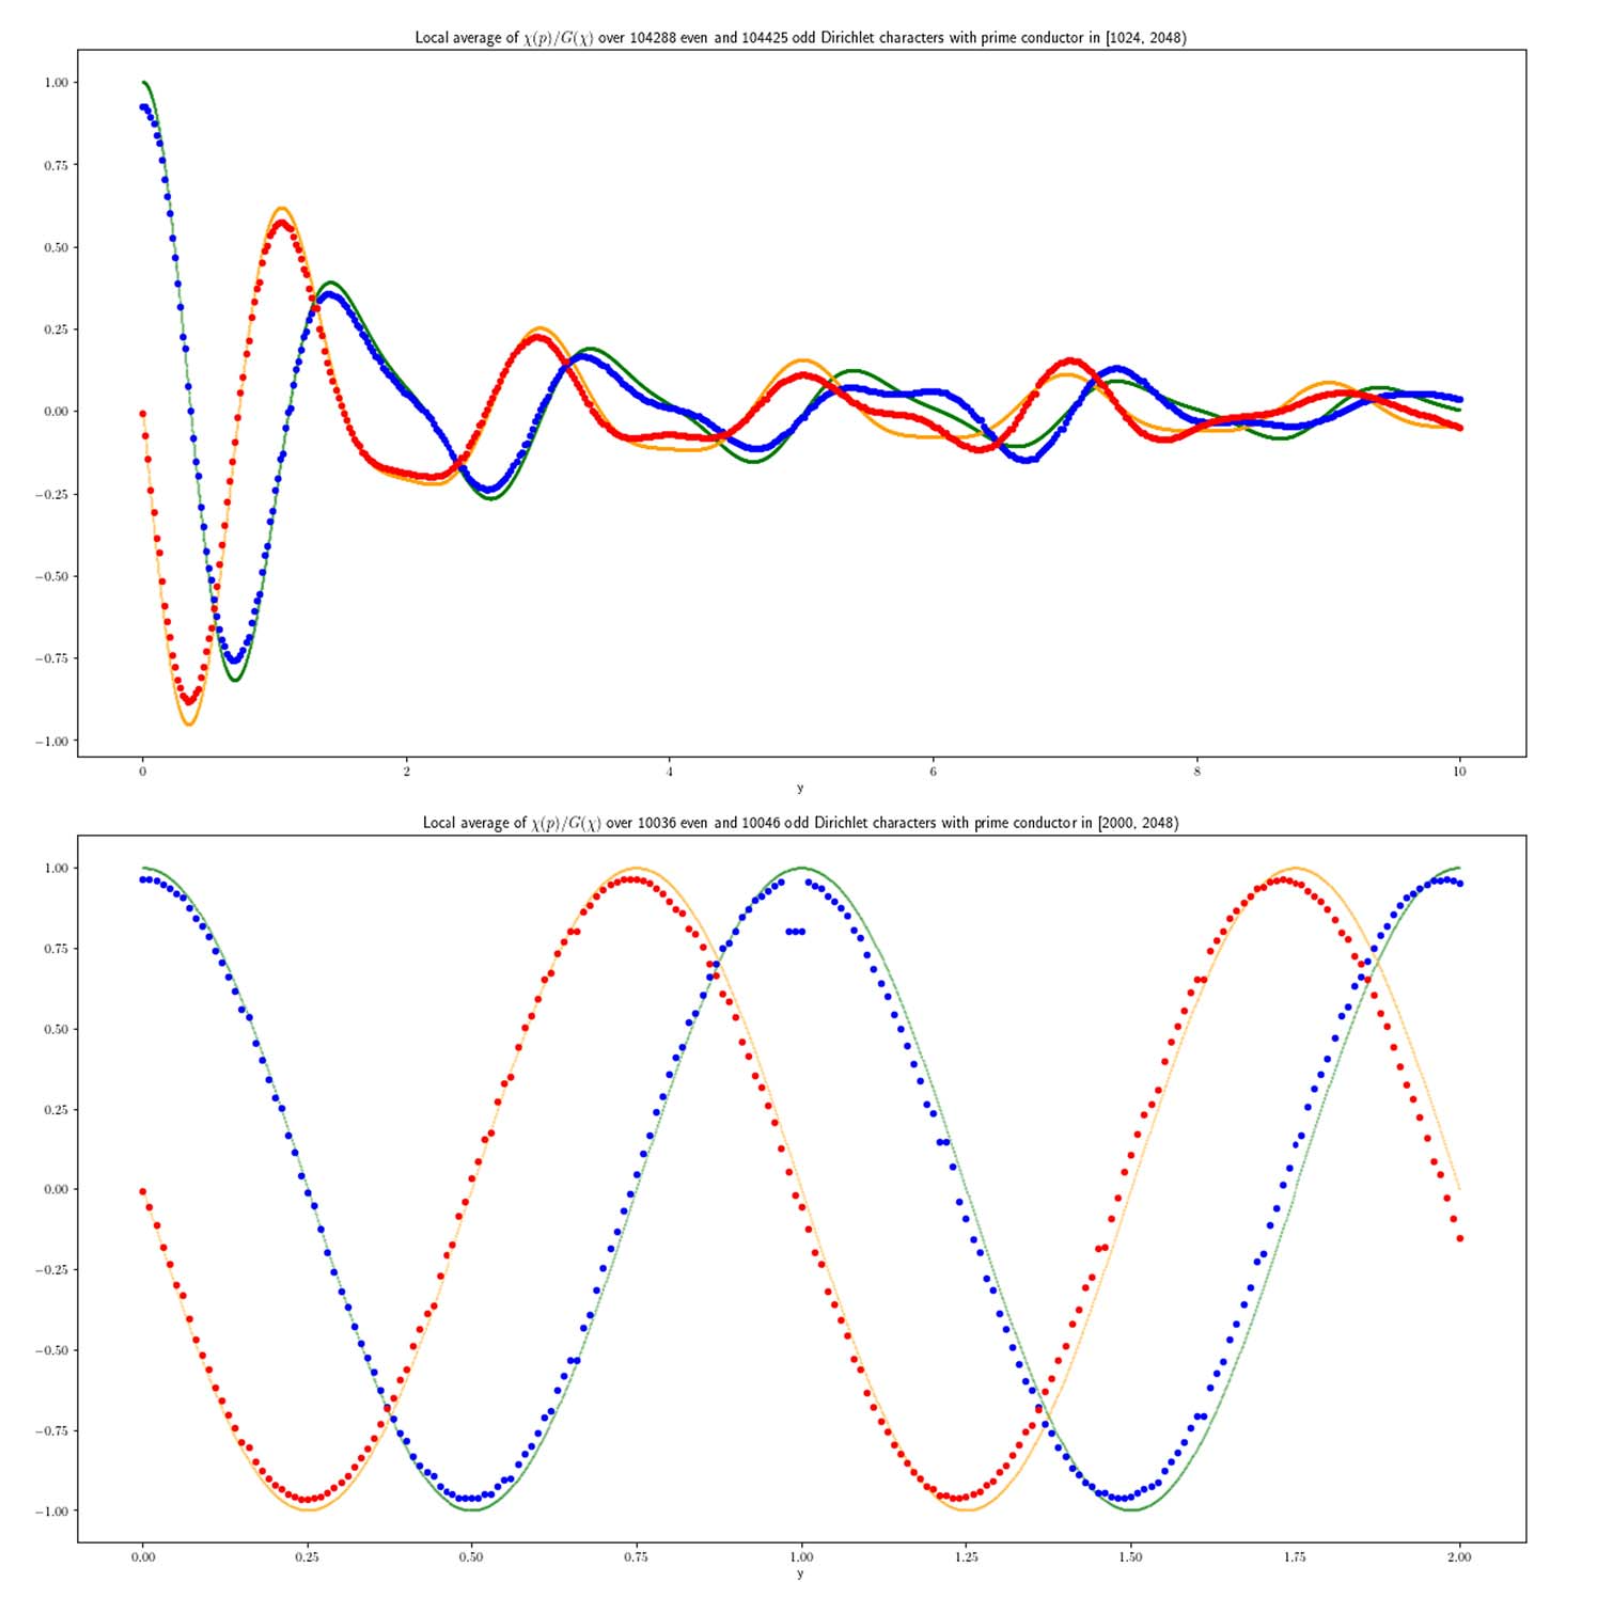
\includegraphics[width=0.7\textwidth]{src/lop.png}%
    \caption{Murmuration of Dirichlet characters. The top figure presents $P_{\pm}(y, 2^{10}, 2)$ for $y \in [0, 10]$ with $+$ in blue and (the imaginary part of) $-$ in red. The bottom figure presents $\widetilde{P}_{\pm}(y, 2002, 0.51)$ for $y \in [0, 2]$ with $+$ in blue and (the imaginary part of) $-$ in red. The discontinuity of $\widetilde{P}_{+}(y, 2002, 0.51)$ at $y = 1$ corresponds to the term $p = N$ in \eqref{eqn:lee_2_avg}.}
\label{fig:lop}
\end{figure}